\chapter{Dataset}

This chapter describes the used datasets, presenting their construction methodology and a brief descriptive analysis.

\section{End-to-End Packet Loss Fraction Time Series Dataset}

\subsection{Methodology}

The time series presented in this work represent network end-to-end measures of a cable-television infrastructure running DOCSIS, with asymmetric download and upload bandwidths. Home routers connected to the cable modem communicates with one or more servers strategically located by the ISP. Measurement results from each home router are consolidated every half hour and, by the end of every day, are transferred to a database for analysis. The software responsible for these procedures was developed by TGR in partneship with UFRJ. 

The focus of this work is to analyze the loss fraction, however, \cite{a_preliminary_performance_measurement_study_of_residential_broadband_services_in_brazil} presents a further analysis on other metrics, such as link throughput, round trip latency and loss bursts. To measure the round trip packet loss fraction between the home router and the associated server, the home router sends a train of short UDP packets, and then the server bounces back them. The data presented here considers a train of 100 UDP packets of 32 bytes and 1 milliseconds apart.

The resulted time series are unevenly due to a range of reasons. One of them is that measurements are initiated only if the residential link is not under use by the ISP customer. Also, it is possible to the home router be without Internet access to start a measurement, or even without electrical energy.

\subsection{Descriptive Analysis}

The TGR software run in a subset of the ISP customers in several brazilian states. In the analysis of this section, it was considered the period from 01/may/2016 to 20/may/2016. It was selected every client in which all measures of this period occurred against the same server. Another imposed constraint was that the home router and the server must belong to the same state. This filter resulted in 1870 clients time series and the total of 1537272 measures.

In figure \ref{fig:loss_fraction_cdf_ccdf} is presented the packet loss fraction CDF and CCDF of all time series. It is possible to note that 93.2\% of the measures have zero losses.

\begin{figure}[H]
    \makebox[\linewidth][c]
    {
        %
        \centering
        \begin{subfigure}[b]{0.55\textwidth}
            \centering
            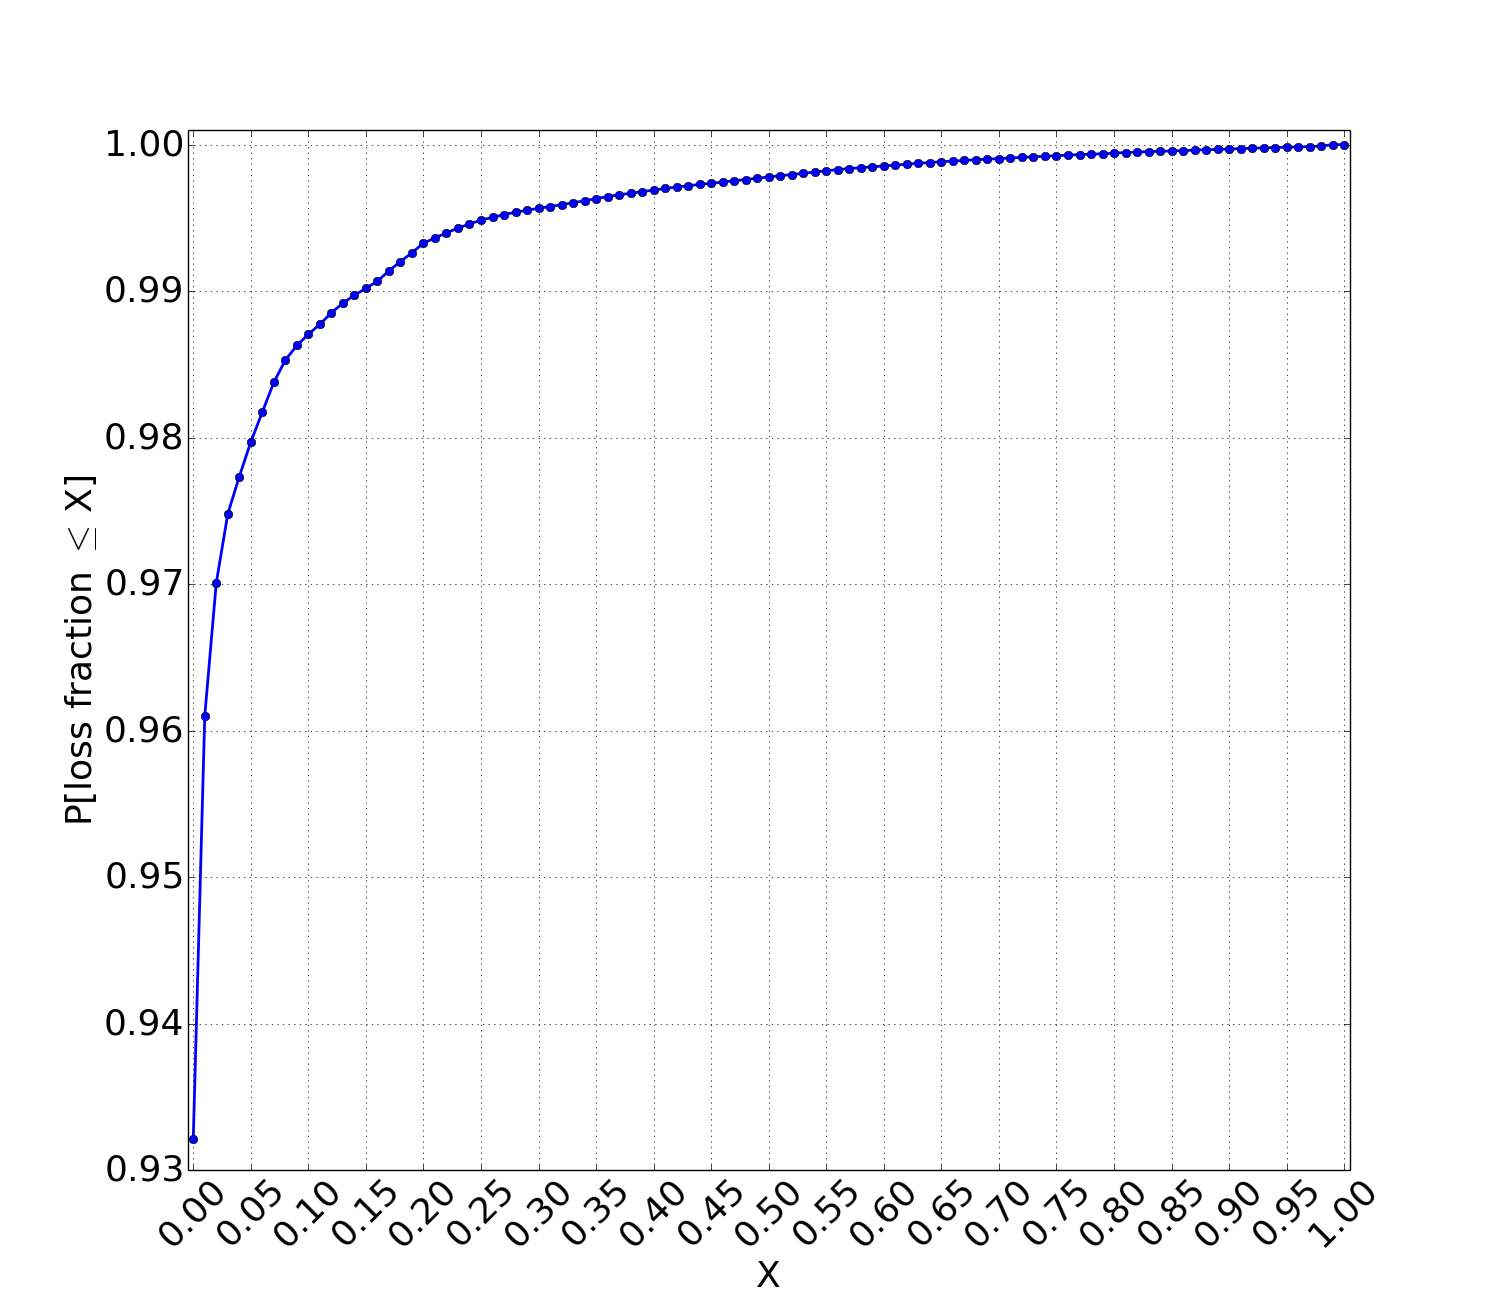
\includegraphics[width=\linewidth]{./figures/loss_cdf.png}
            \caption{CDF}
        \end{subfigure}%
        ~ 
        \begin{subfigure}[b]{0.55\textwidth}
            \centering
            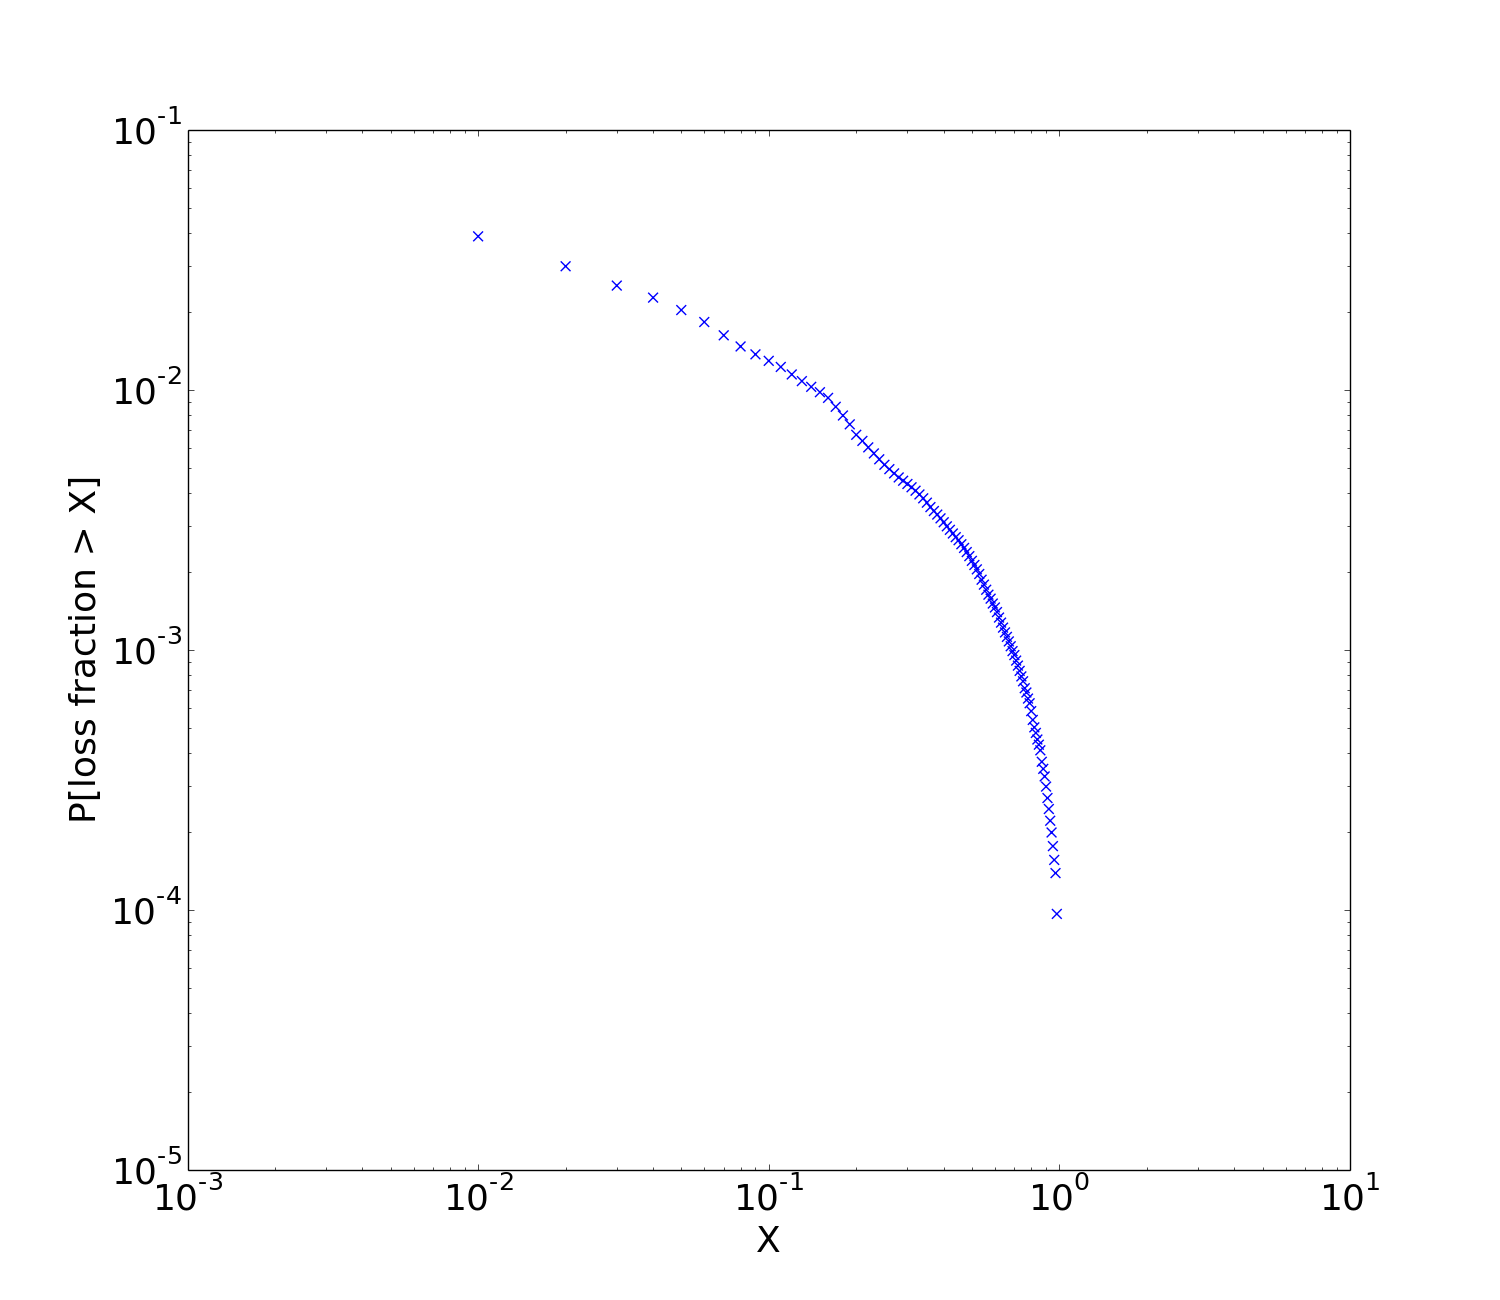
\includegraphics[width=\linewidth]{./figures/ccdf.png}
            \caption{CCDF in log-log scale}
        \end{subfigure}
    }
    \caption{Packet Loss Fraction}
    \label{fig:loss_fraction_cdf_ccdf}
\end{figure}%

Figures \ref{fig:loss_fraction_acf_ts_1}, \ref{fig:loss_fraction_acf_ts_2}, \ref{fig:loss_fraction_acf_ts_3} are three examples of common autocorrelation patterns in this dataset. Since the time series are unenvely, it was considered only the date and hour components of a measure time to compute the autocorrelation function, ignoring then the minutes and seconds information. Therefore, if more than one measure occurred at the same hour and date, it was taken the average of these samples.

\begin{figure}[H]
    \makebox[\linewidth][c]
    {
        %
        \centering
        \begin{subfigure}[b]{0.55\textwidth}
            \centering
            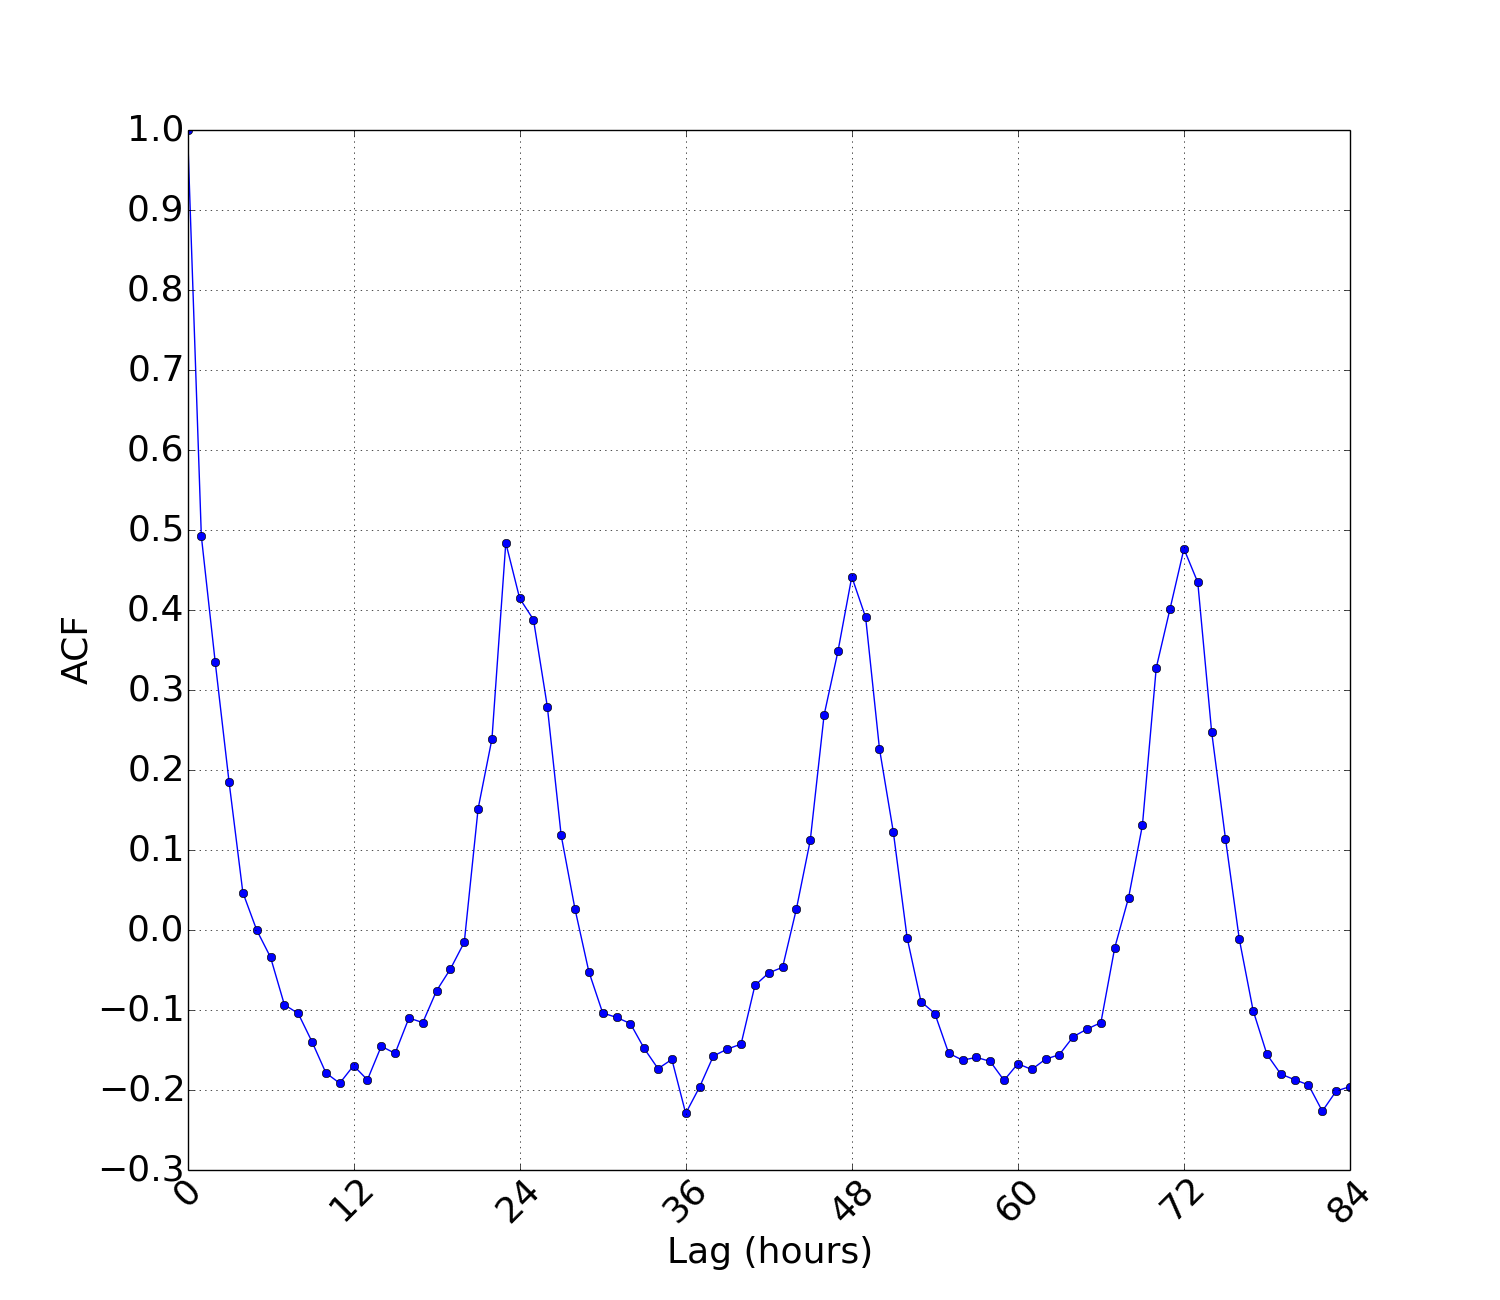
\includegraphics[width=\linewidth]{./figures/acf_NHODTCSRV04_64:66:B3:50:05:BC.png}
            \caption{Autocorrelation}
        \end{subfigure}%
        ~ 
        \begin{subfigure}[b]{0.55\textwidth}
            \centering
            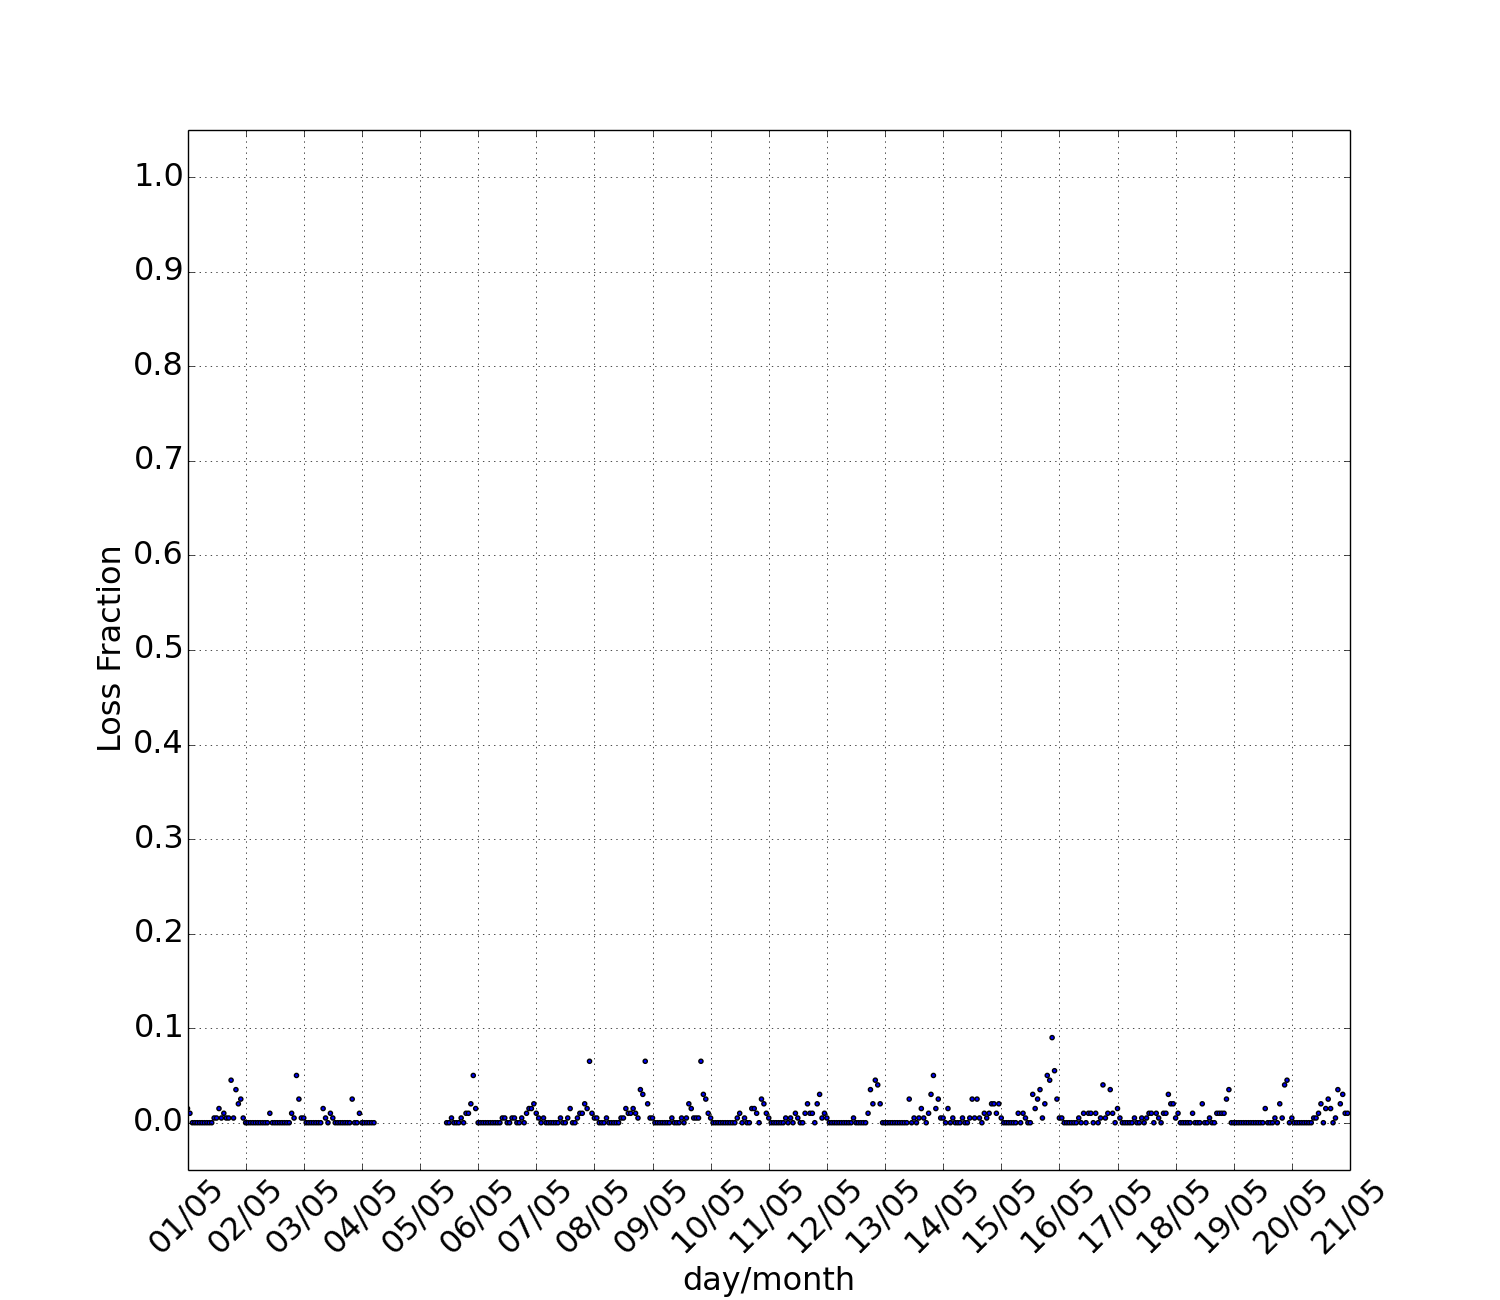
\includegraphics[width=\linewidth]{./figures/ts_NHODTCSRV04_64:66:B3:50:05:BC.png}
            \caption{Time Series}
        \end{subfigure}
    }
    \caption{Client 1}
    \label{fig:loss_fraction_acf_ts_1}
\end{figure}%

\begin{figure}[H]
    \makebox[\linewidth][c]
    {
        %
        \centering
        \begin{subfigure}[b]{0.55\textwidth}
            \centering
            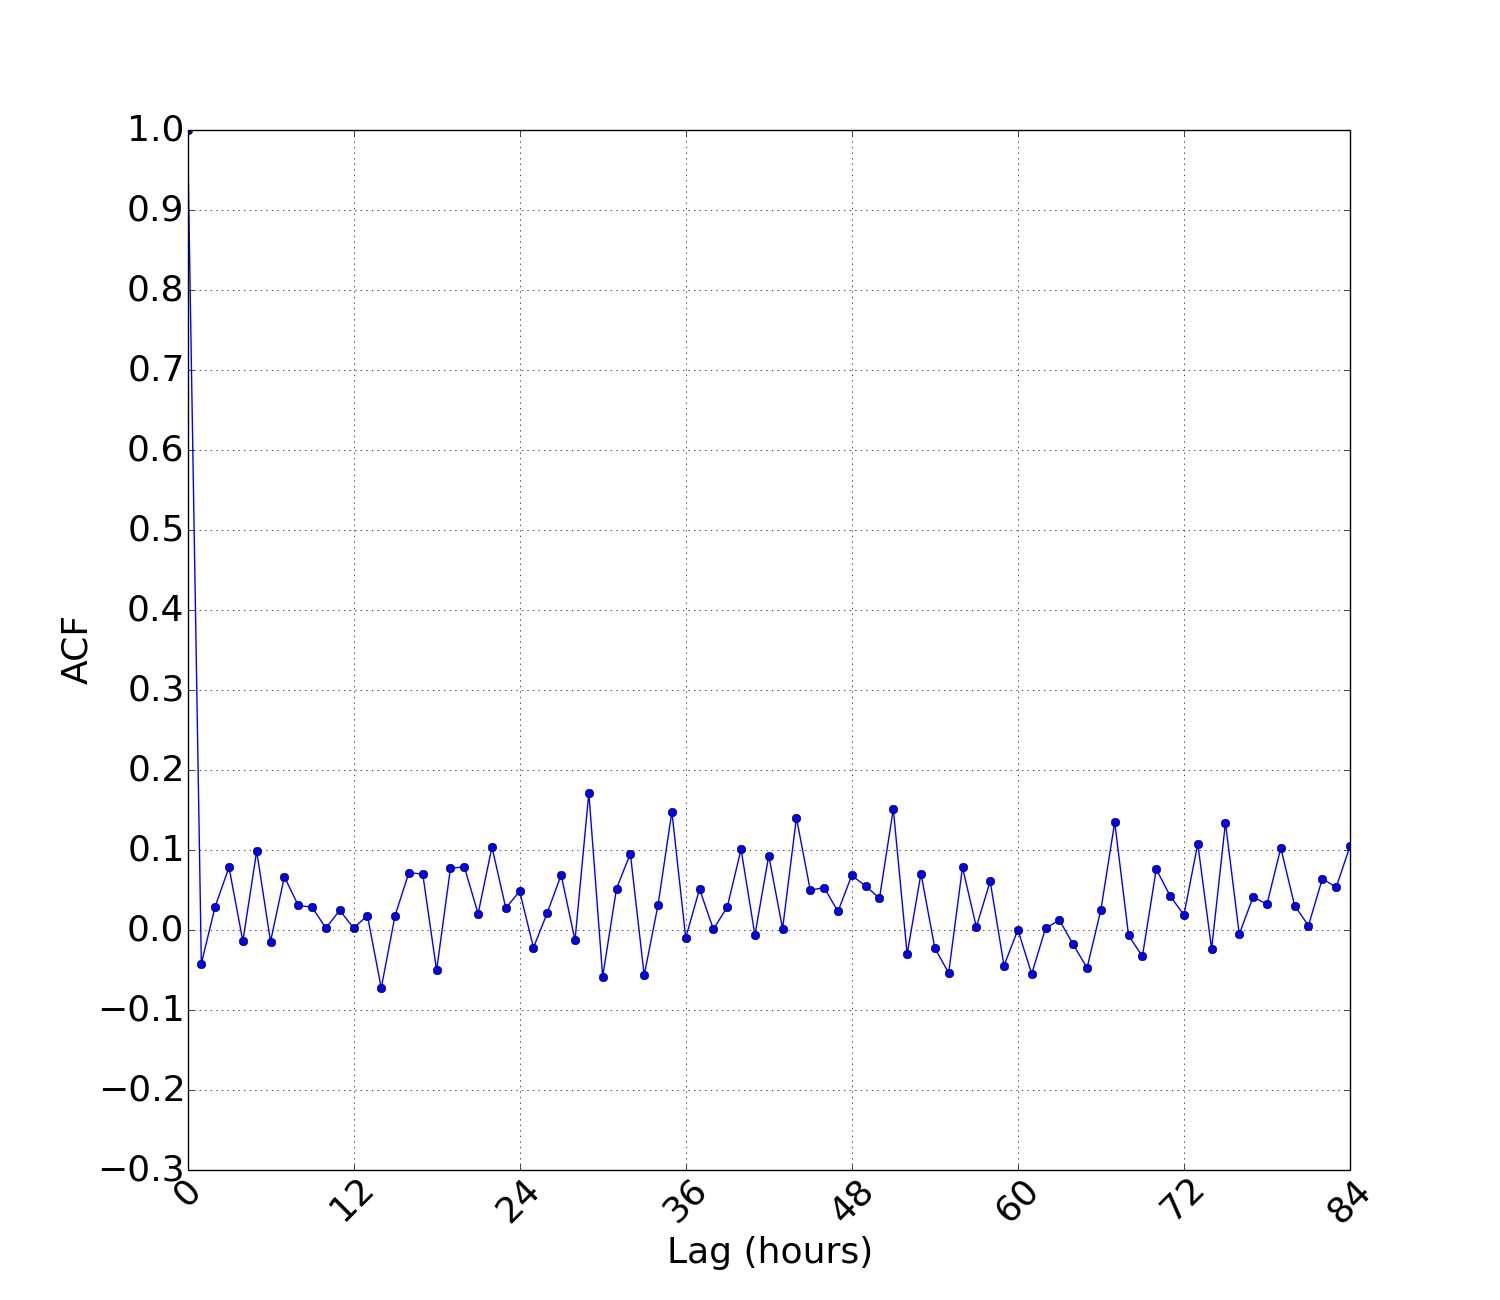
\includegraphics[width=1.0\textwidth]{./figures/acf_BREDTCSRV20_64:66:B3:7B:9E:6A.png}
            \caption{Autocorrelation}
        \end{subfigure}%
        ~ 
        \begin{subfigure}[b]{0.55\textwidth}
            \centering
            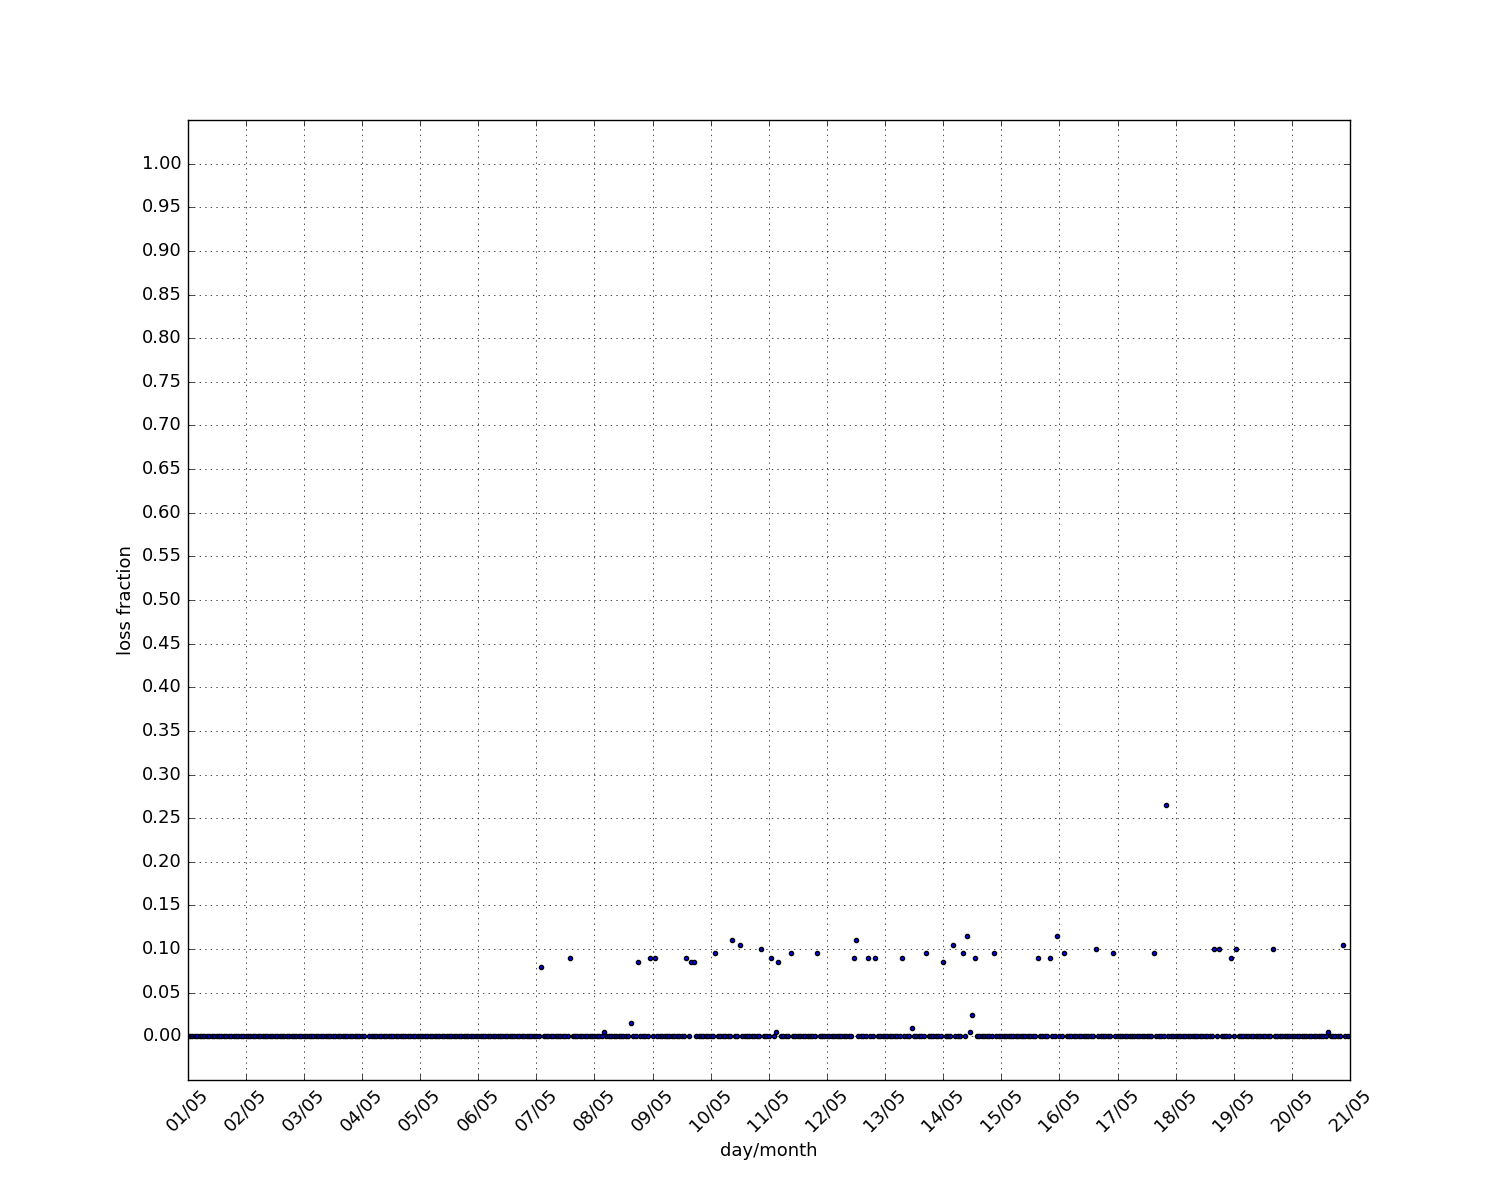
\includegraphics[width=1.0\textwidth]{./figures/ts_BREDTCSRV20_64:66:B3:7B:9E:6A.png}
            \caption{Time Series}
        \end{subfigure}
    }
    \caption{Client 2}
    \label{fig:loss_fraction_acf_ts_2}
\end{figure}

\begin{figure}[H]
    \makebox[\linewidth][c]
    {
        %
        \centering
        \begin{subfigure}[b]{0.55\textwidth}
            \centering
            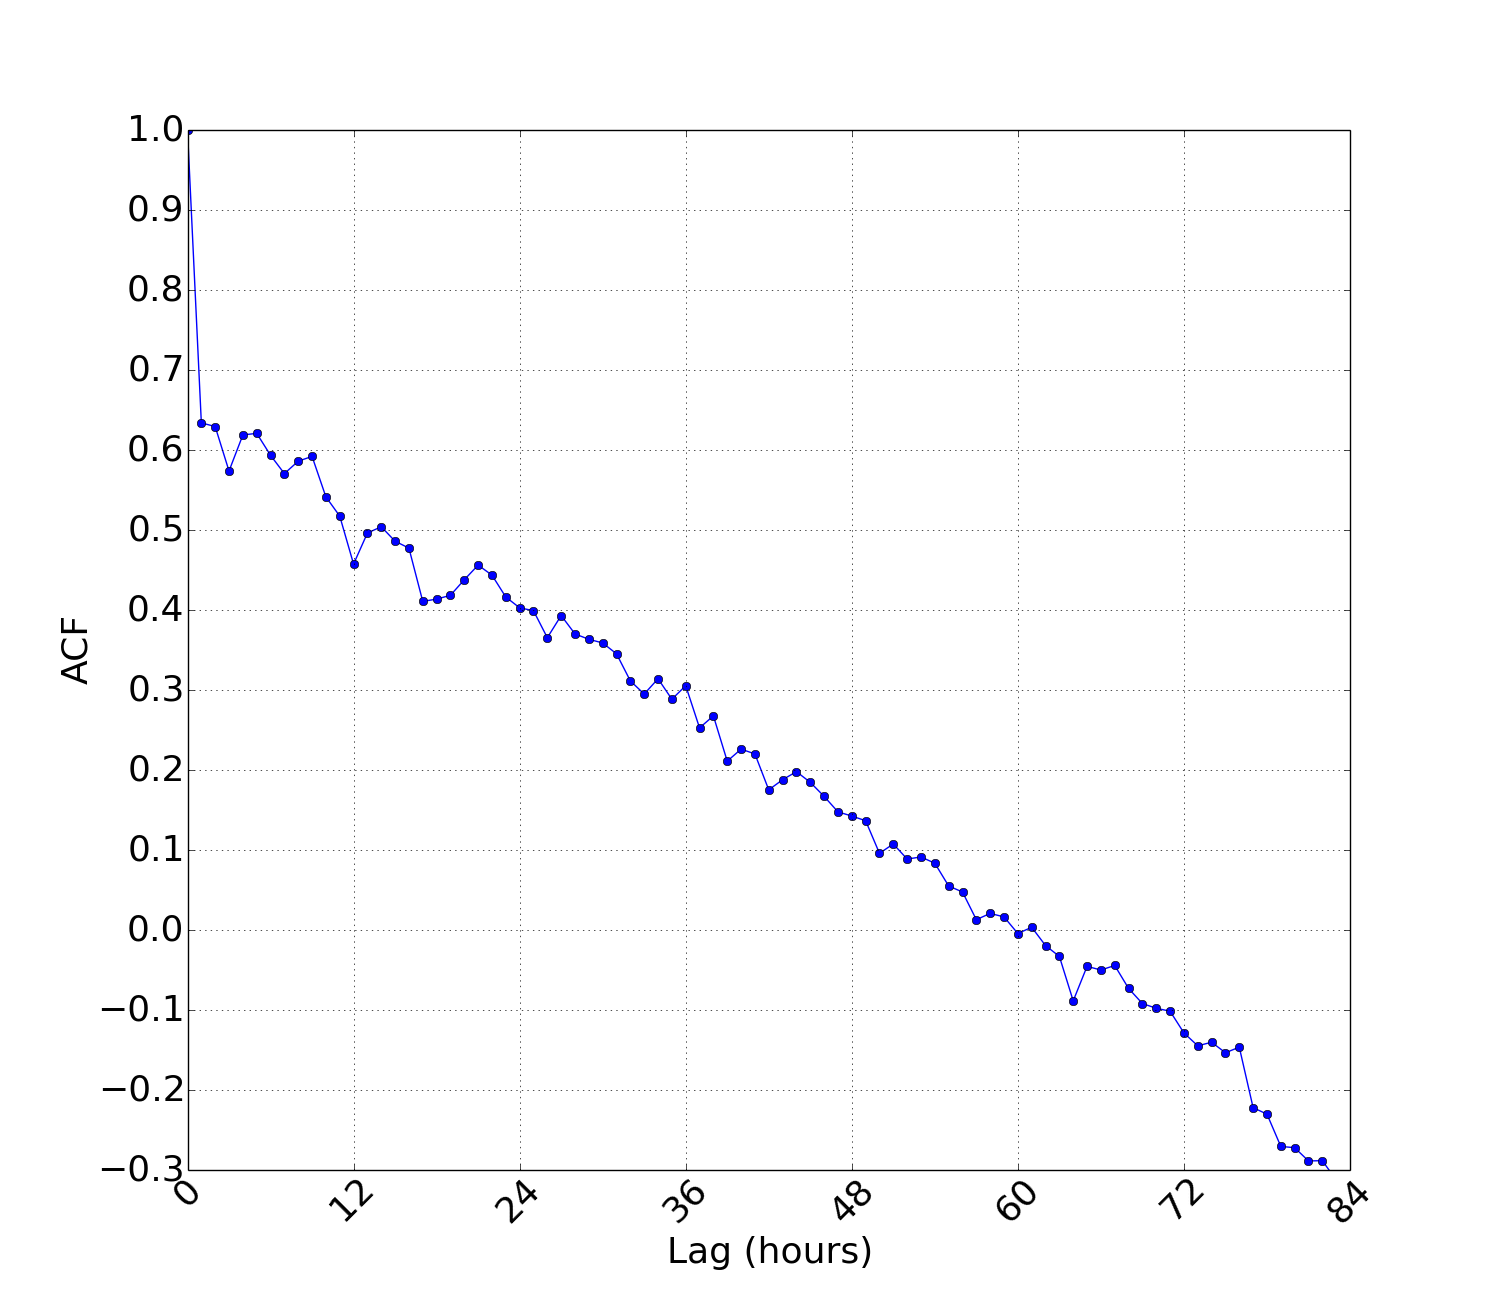
\includegraphics[width=1.0\textwidth]{./figures/acf_BHZRENPEV01_64:66:B3:A6:BA:54.png}
            \caption{Autocorrelation}
        \end{subfigure}%
        ~ 
        \begin{subfigure}[b]{0.55\textwidth}
            \centering
            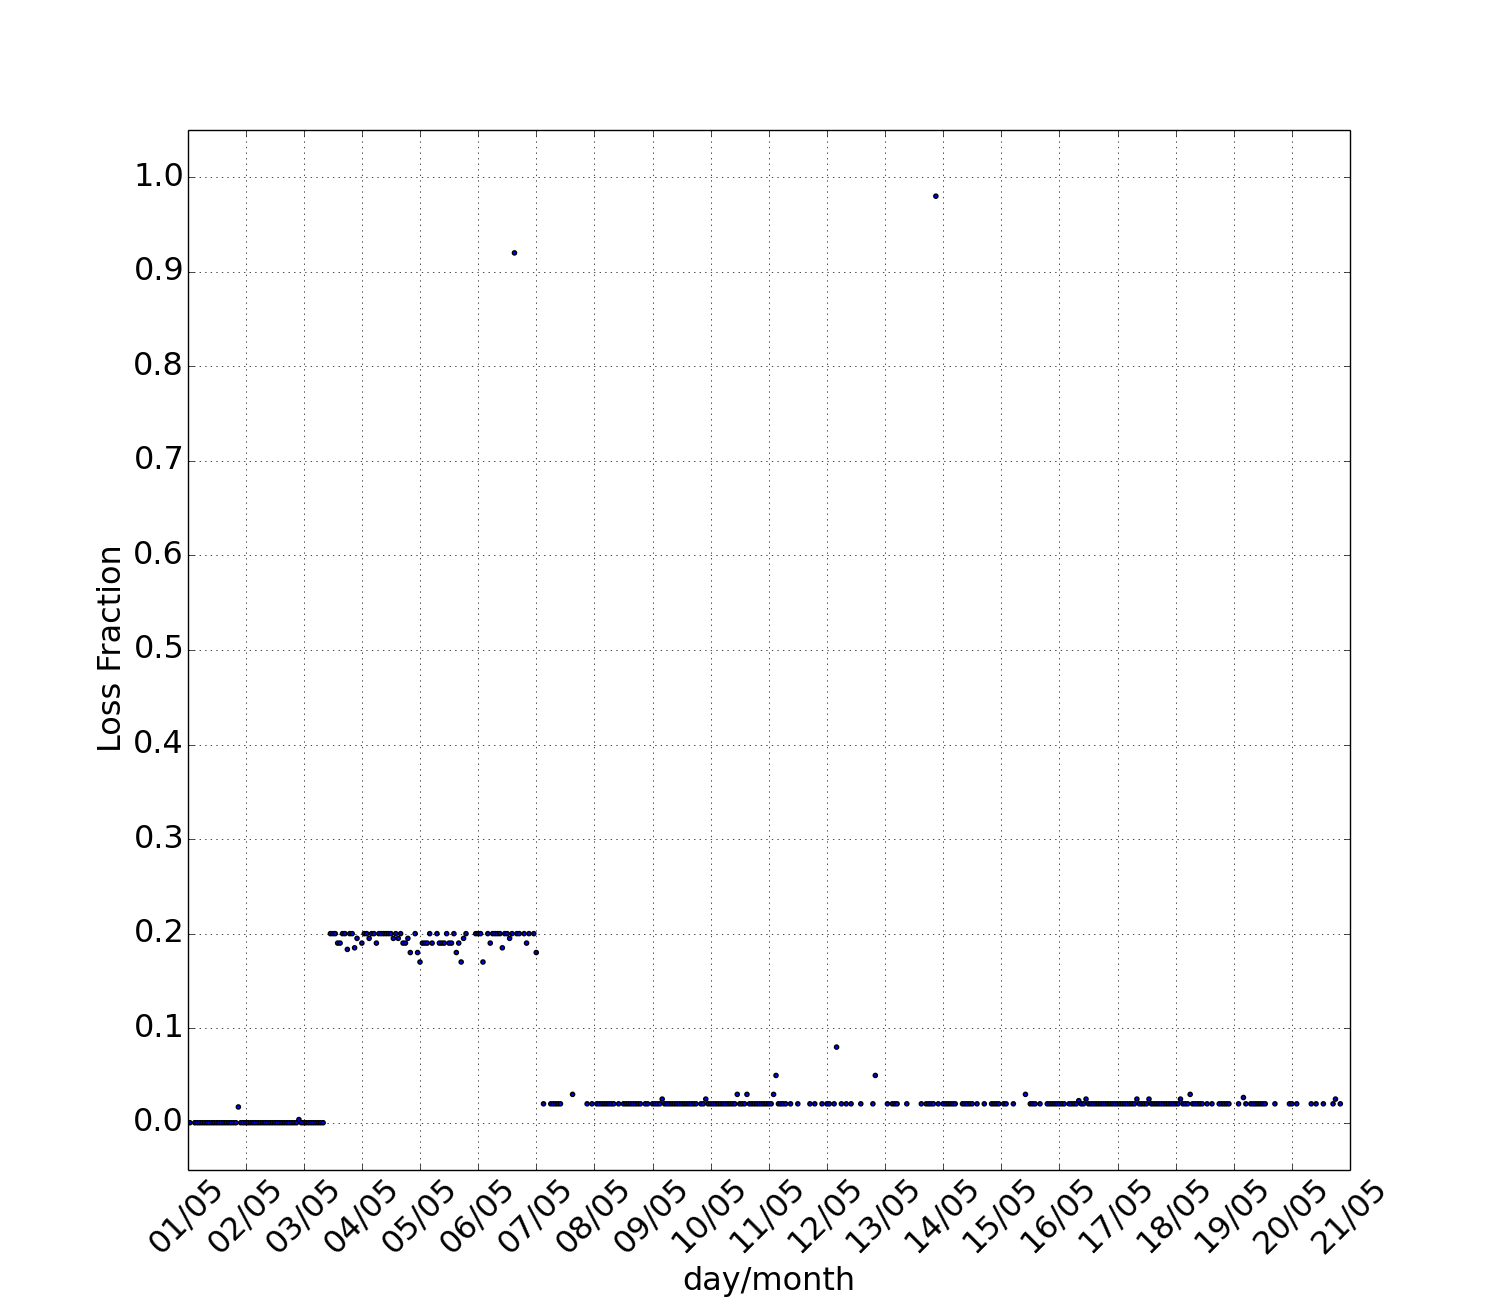
\includegraphics[width=1.0\textwidth]{./figures/ts_BHZRENPEV01_64:66:B3:A6:BA:54.png}
            \caption{Time Series}
        \end{subfigure}
    }
    \caption{Client 3}
    \label{fig:loss_fraction_acf_ts_3}
\end{figure}

The autocorrelation of figure \ref{fig:loss_fraction_acf_ts_1} have a periodic pattern, with peaks around multiples of 24 hours. In this client, it is possible to observe that losses a more usual at night. However, in figure \ref{fig:loss_fraction_acf_ts_2}, the autocorrelation quickly decreases and fluctuates around zero. The corresponding time series have a common characteristic, from 06/may on measures with losses alternated with zero losses measures. Figure \ref{fig:loss_fraction_acf_ts_3} shows a linear decreasing autocorrelation, and the associated time series presents abrupts changes in the mean. 

As in figure \ref{fig:loss_fraction_acf_ts_1}, some clients have a daily pattern in which losses occur more frequently at night. This fact can b in which the Internet usage is known to be bigger. Figure~\ref{fig:mean_day_hour_ts} corroborates that observation, which presents the mean and variance of the measures that occurred in a specific hour during the 20 days period. This can be a indication of congestion during peak of usage hours.

\begin{figure}[H]
    \makebox[\linewidth][c]
    {
        %
        \centering
        \begin{subfigure}[b]{0.55\textwidth}
            \centering
            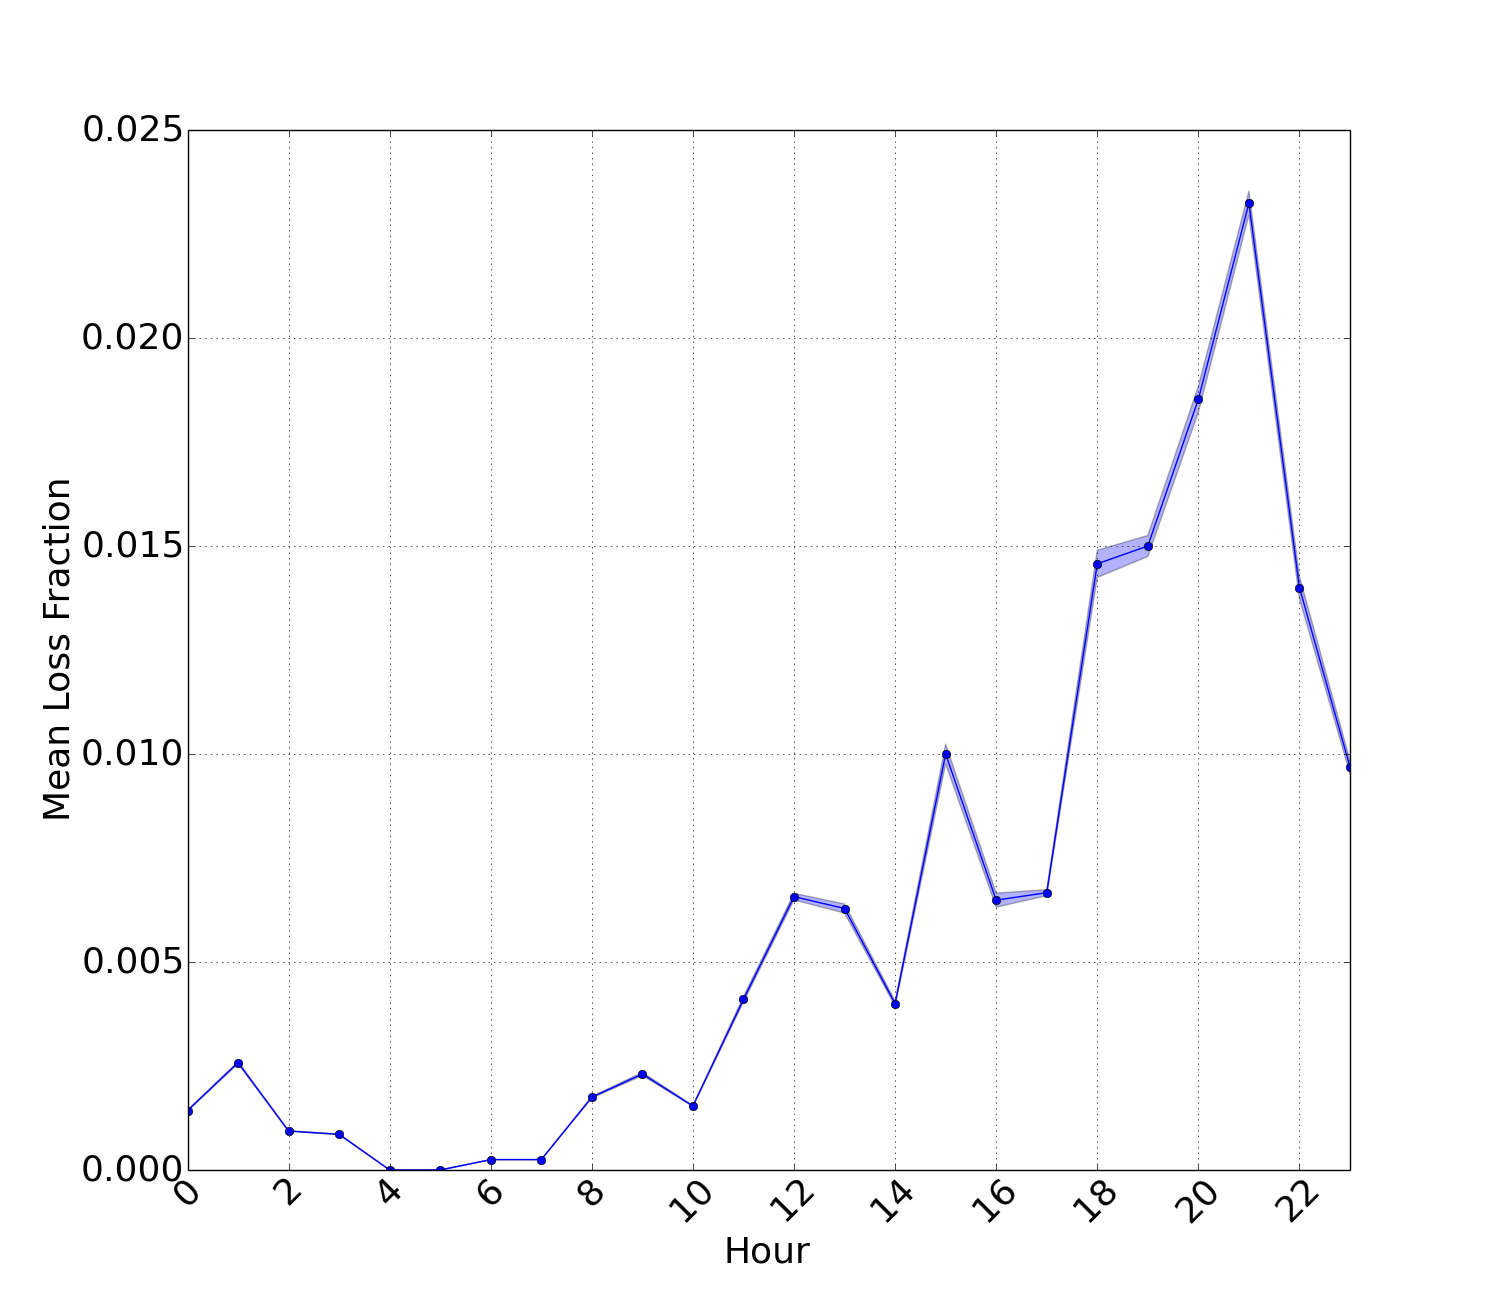
\includegraphics[width=1.0\textwidth]{./figures/mean_per_hour_in_a_day_NHODTCSRV04_64:66:B3:50:06:90.png}
            \caption{Mean and variance per hour}
        \end{subfigure}%
        ~ 
        \begin{subfigure}[b]{0.55\textwidth}
            \centering
            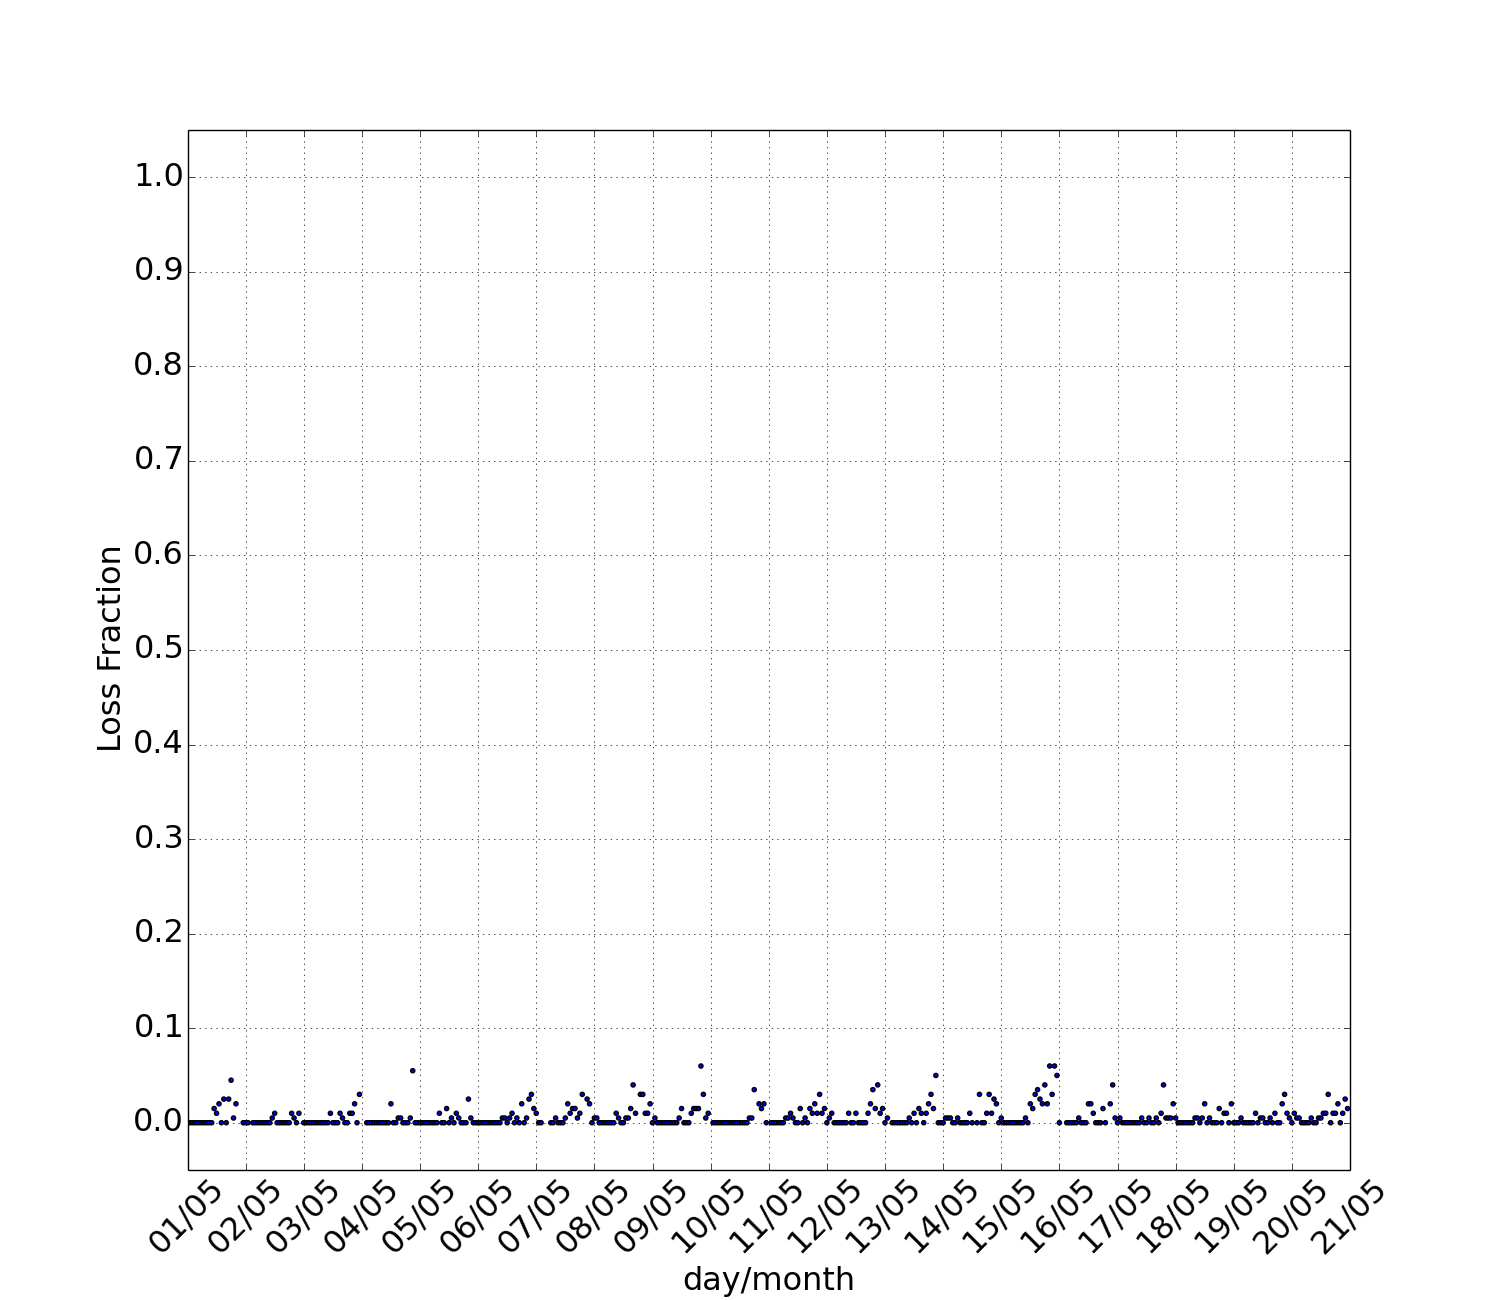
\includegraphics[width=1.0\textwidth]{./figures/ts_NHODTCSRV04_64:66:B3:50:06:90.png}
            \caption{Time Series}
        \end{subfigure}
    }
    \caption{Client 1}
    \label{fig:mean_day_hour_ts}
\end{figure}

Also, through a visual analysis, as in the previous figures, it is possible to observe different time series and change points patterns.

% - mean loss by week day of single client\\
% - power spectra to check periodicity? \\

\section{Change Points Dataset}

There are several approaches to construct a change points dataset to test a change point detection method. Some works in the literature simply create a simulated time series thorugh generative models, however different segments are generated by the same model but with different parameters. In general, this types of time series are more easily handled in change point detection algorithms, since some methods assumes the same models that generated the data or because real data can have more complex characteristics. Another way is to create a time series appending different segments provenient from different real time series data. In this cases is easy to simplify the dataset since some characteristics as the segments lengths are defined by the dataset creator and another ones are fakely introduced. Another works assumes that the latent information of the time series are available, and with specific knowledge of the application field, it is possible to assume what kinds of configuration changes could induce a change in the time series. In the case of the application field of the present work this would be difficult, since the latent information would be connected with the network situation such as network topology, characteristics of routers congestions, physical equipments problems, which is a too complex, or even impossible information to collect and also to assume which variables could impact the time series. Other apprach also uses the latent information but instead creates a controlled environment in which is possible to change the configuration over time, but as in the previous case, this would be too complex. The approach followed by this work was to use a visual annotation of the time series. It were conducted, with an application domain specialist, visuallyu indicating the relevant changes. It is known that human visual inspection methods can bring erroneous conclusions, but with the data and application scenarion it was the best fit, as network engineers visually identify, after simple automatic filters, the change points.

This work is interested in work directly with real data and satisfy a real application problem.

As in other tasks, it is difficult to translate a human visual perception in a sistematically method.

In general, when the exact types of target changes are previously know the problem is easier.

\section{Methodology}

It was created an annotation system to a specialist visually indicates the change points of the time series dataset. The user indicated with the mouse the points in time where he thinks that where the cahnge points occurred. To avoid results misunderstanding X axis of the time series represented onlu the time order of the measures, since the time series are unevenly this fact could visually wrong infer change points. Also, since is known that variances in the losses fractions when the losses are low have more impact in the user QoE than when the losses are big, the system also provides two other y scales than linear, the log scale and piecewise linear with bigger length in [0, 0.1] than (0.1, 1.0]. The user can click in any scale.

A single person classified all time series. This person has experiences with academic and industry network measurements and statistical modelling, however without background in change point detection analysis. The user could take the time he wants to make a classification and it was able to classify in different days. Before the user could start the classifications, it was indicated a series of instructions: 

\begin{itemize}
    \item In the case of packet loss fraction, mean changes between 0 and 0.1 are more sensible to the end users.
    \item The "time" axis only represents the temporal order of the measurements. However, in general, consecutive points in "time" axis are separated by 30 minutes.
    \item Outlier is not a statistical change. An outlier is an observation that lies outside the overall pattern of a distribution.
\end{itemize}

Since several time series of the previously described time series have almost all measures with zero losses, these time series was filtered to reduce the number of time series and keep only the ones which provide change points, increasing the entropy. Also, to better the visualization, it was selected time with 10 days of data, therefore the dataset consists of time series from 1 may 2016 to 10 may 2016, and from 11 may 2016 to 20 may 2016. The specific filter was: it was selected only the time series that has 85\% of the maximum possible data in the specified time period, considering that each home router executes the measurement procedure at most two times in a hour. Reducing to 522 time series. Also it were only selected the time series that have at least one window of length 48 with at least 6 measures with loss fraction bigger than 0.01.

\section{Descriptive Analysis}

- explain possible ways to get the ground truth\\
- description of the volunteer\\
- user instructions\\
- snapshots of system\\ 
- how time series were selected to be in the survey\\

\section{Description of Change Points Dataset}

- number of time series, number of change points: it is a high dimensional problem\\
- distribution number of changes per time series\\
- distribution time between change points\\
- distribution time for the first change point\\
- distribution time from last change point to time series end\\
- distribution of classification time?\\
- measure the difference between consecutive segments?\\

\section{Performance Evaluation}

- how the performance is asserted in literature\\
- ROC curve\\
- confusion matrix and accuracy metrics\\
